\documentclass[graybox]{svmult}


\usepackage[T1]{fontenc}

% The editors specifically asked for Lucida Console.
% Hence, I switched to XeLaTeX. This does, of course,
% not work with PDFLaTeX. You'll know how to go back
% to PDFLaTeX if you have to.
\usepackage{fontspec}
\setmonofont[Scale=0.9]{Lucida Console}

\usepackage{makeidx}
\usepackage{multicol}
\usepackage[bottom]{footmisc}
\usepackage{newtxtext}
\usepackage{newtxmath}

\usepackage{xcolor}
\definecolor{lightgray}{gray}{0.85}
\usepackage{listings}
\lstset{%
  language=R,
  keywordstyle=\color{black},
  basicstyle=\ttfamily\small,
  backgroundcolor = \color{white},
  frame=trbl,
  rulecolor=\color{white},
  framesep=10pt,
  xleftmargin=10pt,
  xrightmargin=10pt
}

\usepackage[hyphens]{url}

\usepackage{hhline}
\usepackage{booktabs}
\usepackage{colortbl}
\usepackage{gb4e-}
\usepackage[xetex]{graphicx}

\usepackage[backend=biber,
	natbib=true,
	style=bst/unified/bbx/biblatex-sp-unified,
	citestyle=bst/unified/cbx/sp-authoryear-comp,
	maxbibnames=99,
	isbn=false,
	doi=false,
	eprint=false
]{biblatex}
\bibliography{glmm}

%\usepackage{natbib}
%\bibliographystyle{styles/spbasic}


\newcommand{\Lf}{
  \setlength{\itemsep}{1pt}
  \setlength{\parskip}{0pt}
  \setlength{\parsep}{0pt}
}

\newcommand{\wrt}{w.\,r.\,t.\ }
\newcommand{\ie}{i.\,e.,\ }
\newcommand{\Ie}{I.\,e.,\ }
\newcommand{\eg}{e.\,g.,\ }
\newcommand{\Eg}{E.\,g.,\ }
\newcommand{\Aa}{The author\ }
\newcommand{\A}{the author\ }

\newcommand{\Sub}[1]{\ensuremath{\mathrm{_{#1}}}}
\newcommand{\Sup}[1]{\ensuremath{\mathrm{^{#1}}}}
\newcommand{\vivs}{VI\slash VS\ }

\newcommand{\Rformula}[3]{\begin{equation}{\texttt{#1\textasciitilde #2}}\label{#3}\end{equation}}

\title{Mixed-effects regression modeling}
\author{Roland Schäfer}
\institute{Roland Schäfer \at Deutsche und niederländische Philologie, Freie Universität Berlin \email{roland.schaefer@fu-berlin.de}}

\begin{document}       

% To make it look right to LaTeX-unaware editors.
\setcounter{chapter}{21}
\renewcommand*\thesection{\arabic{section}}

\maketitle

\section{Introduction}
\label{sec:introduction}

Mixed effects modeling is an extension of (generalised) linear modeling, of which logistic regression (see Chapter 21) is an instance.
A common characterisation of mixed-effects modeling is that it accounts for situations where observations are \textit{clustered} or \textit{come in groups}.
In corpus linguistics, there could be clusters of observations defined by individual speakers, registers, genres, modes, lemmas, etc.
Instead of estimating coefficients for each level of such a grouping factor (so-called \textit{fixed effects}), in a mixed model it can alternatively be modeled as a normally distributed random variable (a so-called \textit{random effect}) with predictions of group-wise tendencies being made for each group.
This chapter introduces readers to the situations where mixed-effects modeling is useful or necessary.
The proper specification of models is discussed, as well as some model diagnostics and ways of interpreting the output.
Readers are assumed to be familiar with the concepts covered in the previous chapter.

\section{Fundamentals}
\label{sec:fundamentals}

\subsection{When are random effects useful?}
\label{sec:whenrandomeffectsareuseful}

In (Generalised) Linear Mixed Models (GLMMs) -- or, more generally speaking, ``multilevel models'' or ``hierarchical models'' (see \citealp{GelmanHill2006} and Section~\ref{sec:hierarchicalormultilevelmodels} below) -- the purpose of including random effects is usually said to be the modeling of variance between groups of observations.
A single observation (alternatively ``data point'', ``measurement'', or ``unit'') is one atomic exemplar entering into the statistical analysis of a study.
In corpus linguistics, single observations can be understood as single lines in a concordance.
These concordance lines could contain, for example, clauses or sentences in which one of the alternants of a morpho-syntactic alternation occurs, the goal being to model the influence of diverse properties of the clauses or sentences on the choice of the alternants.
Along similar lines, they could contain occurrences of a contracted or a non-contracted form of words (like \textit{am} and \textit{'m} in English).
As another example, the concordance lines could contain NPs where two pre-nominal adjectives are used, the goal being to determine the factors influencing their relative ordering.
When such observations are grouped, it is often plausible to assume that there is some variance in the choice of the alternating forms or constructions at the group-level (such as the level of the individual speakers, registers, lemmas, etc.).

Groups can be defined by any linguistically relevant grouping factor, such as the individual speakers (or authors, writers, etc.), the regions where they were born or live, social groups with which they identify, but also time periods, genres, styles, etc.%
\footnote{Trivially, grouping factors should never be ordinal variables.
The are always categorical.
Terminologically, the ``groups'' are the collections of observations, and each such group corresponds to the ``levels'' of the categorical grouping factor.}
Specific lexemes often have idiosyncratic affinities towards alternants in alternating constructions.
Therefore, exemplars containing specific lexemes also constitute groups.
In cases like the dative alternation in English, individual verbs co-occur with the alternants to different degrees.

If this is the case and the grouping factor is not included in the model, the error terms within the groups will be correlated.
Put simply, the error terms would have a certain tendency per group.
We would find group-wise tendencies, for example, if sentence length were modeled (for example using the types of constructions or lexemes occurring in it) and individual speakers represented in the data had tendencies to form longer or shorter sentences.
If the speaker variable were not included as a predictor in the model under such conditions, the model would make predictions averaged over all speakers, and for short-sentence speakers, these predictions would tend to be too high, whereas for long-sentence speakers, they would be too low.
However, the algorithms used for estimating the parameters of GLMs (so-called estimators) work under the assumption of non-correlated errors, an assumption often called ``independence (of errors)''.
Thus, the prediction errors should not have group-wise tendencies as described above.

If the assumption of independence does not hold, standard errors for model coefficients will typically be estimated as smaller than they nominally are, leading to increased Type I error rates in inferences about the coefficients.
This gets even worse when there are within-group tendencies regarding the direction and strength of the influence of the other regressors, \ie when there is an interaction between them and the grouping factor (\eg \citealt{SchielzethForstmeier2009}).
This is why known variation by group should be accounted for in the model.
Random effects are one convenient way to do so with some advantages and disadvantages compared to fixed effects.

The crucial question in specifying models is not whether to include these grouping factors at all, but rather whether to include them as fixed effects or as random effects.
Random effect structures are very suitable for accounting for group-level variation in regression, but formulaic recommendations such as ``Always include random effects for speaker and genre!'' are inappropriate.
The choice between fixed and random effects should be made based on an analysis and understanding of the data set at hand and the differences and similarities in the resulting models.
The remainder of Section~\ref{sec:whenrandomeffectsareuseful} introduces three important points to consider about the structure of data sets in this context.
Then, Section~\ref{sec:modelspecificationandmodelingassumptions} provides a moderately technical introduction to the actual modeling.


\subsubsection{Crossed and nested effects}
\label{sec:crossedandnestedeffects}

\begin{table}
  \centering
  \begin{tabular}{lll}
    \toprule
    \textbf{Exemplar} & \textbf{Speaker}  & \textbf{Region}        \\
    \midrule
                    1 &           Daryl  &         Tyneside       \\
                    2 &           Daryl  &         Tyneside       \\
                    3 &           Riley  &         Tyneside       \\
                    4 &           Riley  &         Tyneside       \\
                    5 &           Dale   &         Greater London \\
                    6 &           Dale   &         Greater London \\
                    7 &           Reed   &         Greater London \\
                    8 &           Reed   &         Greater London \\
    \bottomrule
  \end{tabular}
  \caption{Illustration of nested factors}
  \label{tab:nested}
\end{table}

This section discusses a distinction that arises when there is more than one grouping factor.
When this is the case, each pair of grouping factors can be ``nested'' or ``crossed''.
By way of example, we can group exemplars (such as sentences) by the individual speakers who wrote or uttered them, and we can group speakers by their region of birth.
Such a data set would intrinsically be ``nested'', as Table~\ref{tab:crossed} illustrates.
Since speakers have a unique region of birth, Tyneside is the unique region value for the speakers Daryl and Riley, and Greater London is the unique region value for Dale and Reed.
In this example, the region factor nests the speaker factor.
This example was chosen because the nesting is conceptually necessary.
However, even when a data set has a nested structure by accident, standard packages in R will also treat them as nested (see Section~\ref{sec:specifyingmodelsusinglme4inr}).

When grouped entities do not uniquely belong to groups of the other grouping factor, the factors are ``crossed''.
Continuing the example, crossed factors for speaker and mode are illustrated in Table~\ref{tab:crossed}.
%
\begin{table}
  \centering
  \begin{tabular}{lll}
    \toprule
    \textbf{Exemplar} & \textbf{Speaker}  & \textbf{Mode}   \\
    \midrule
                    1 &           Daryl  &         Spoken  \\
                    2 &           Daryl  &         Written \\
                    3 &           Riley  &         Spoken  \\
                    4 &           Riley  &         Spoken  \\
                    5 &           Dale   &         Written \\
                    6 &           Dale   &         Written \\
                    7 &           Reed   &         Spoken  \\
                    8 &           Reed   &         Written \\
    \bottomrule
  \end{tabular}
  \caption{Illustration of crossed factors}
  \label{tab:crossed}
\end{table}
%
While there are only spoken sentences by Riley and only written sentences by Dale in the sample, there is one spoken and one written sentence each by Daryl and Reed.
There is a many-to-many relation between speakers and modes, which is characteristic of crossed factors.
In Table~\ref{tab:nested}, the relation between speakers and regions is many-to-one, which is typical of nested factors.

With more than two grouping factors, there can be nesting within nesting, etc.
Mode could nest genre if genres are defined such that each genre is either exclusively spoken or written.
Similarly, in a study on adjectives we might want to describe adjectives as being either intersective or non-intersective.
Within the two groups, a finer-grained semantic classification which itself nests single adjective lexemes might be nested.
However, not all of these structures should be modeled as nested random effects.
In the latter case, for example, the low number of levels of one factor (intersective vs.\ non-intersective) predestines it as a second-level predictor rather than a nesting factor (see Section~\ref{sec:modelspecificationandmodelingassumptions}).

\subsubsection{Hierarchical\slash multilevel modeling}
\label{sec:hierarchicalormultilevelmodels}

This section describes the types of data structures which require the use of multilevel models, which represent a generalisation of the simple mixed effects models discussed so far.
Such data structures are similar or even identical to nested data structures.
Let us assume that we wanted to account for lexeme-specific variation in a study on an alternation phenomenon such as the dative alternation in English by specifying the lexeme as a random effect in the model.
Additionally, we entertain the hypothesis that a lexeme's overall frequency influences its preferences for occurring in the construction alternants.
A similar situation would arise in a study of learner corpus data (even of the same alternation phenomenon) with a learner grouping factor if we also knew that the number of years learners have learned a language influences their performance with regard to a specific phenomenon.
In such cases, variables like the frequency and the number of learning years are constant for each level of the grouping factor (lexeme and learner, respectively).
In other words, each lexeme has exactly one overall frequency, and each learner has had a fixed number of years of learning the language.

\begin{table}
  \centering
  \begin{tabular}{llllll}
    \toprule
    \multicolumn{3}{l}{\textbf{Level of observations}}          & \multicolumn{2}{l}{\textbf{Group level}}  & \textbf{Outcome} \\
    \textbf{Exemplar} & \textbf{Givenness} & \textbf{NP length} & \textbf{Verb} & \textbf{Verb freq.}       & \textbf{Alternant}\\
    \midrule
            1 &     New   &      8    &    give   &   6.99   & 1 \\
            2 &     Old   &      7    &    give   &   6.99   & 1 \\
            3 &     Old   &      5    &    give   &   6.99   & 2 \\
            4 &     Old   &      5    &    grant  &   5.97   & 2 \\
            5 &     New   &      9    &    grant  &   5.97   & 1 \\
            6 &     Old   &      6    &    grant  &   5.97   & 2 \\
            7 &     New   &      11   &   promise &   5.86   & 2 \\
            8 &     New   &      10   &   promise &   5.86   & 1 \\
            9 &     Old   &      9    &   promise &   5.86   & 2 \\
    \bottomrule
  \end{tabular}
  \caption{Illustration of a fictional data set which requires multilevel modeling}
  \label{tab:multilevel}
\end{table}

Such variables are thus interpretable only at the group-level.
Table~\ref{tab:multilevel} illustrates such a data set (fictional in this case).
It might be a small fraction of the data used to predict whether a ditransitive verb is used in the dative shift construction or not.
The NP length is measured in words, the lemma frequencies are actual logarithm-transformed frequencies per one million tokens taken from ENCOW14A \citep{SchaeferBildhauer2012}.
The outcome column encodes whether alternant 1 or 2 was chosen.
As the table shows, the givenness status and the NP length vary at the level of observations.
To capture verb lemma specific tendencies, a verb lemma grouping factor is added.
The verb lemma frequency necessarily varies at the group level because each lemma has a unique frequency.
In such cases, an adequately specified multilevel model uses these so-called ``second-level fixed effects'' to partially predict the tendency of the grouping factor, which is why they are also called ``second-level predictors''.%
\footnote{The fixed effects discussed so far, which are interpreted at the level of observations, are consequently called ``first-level fixed effects'' or ``first-level predictors''.}
Put differently, the idiosyncratic effect associated with a lexeme, speaker, genre, etc.\ is split up into a truly idiosyncratic preference and a preference predictable from group-level variables (such as the frequency of the lemma or the age of the speaker).
In Section~\ref{sec:morecomplexmodels}, it will be explained briefly that in such cases, a second model has to be specified which predicts the group-level tendency from the second-level effects.
The data look similar to multilevel nesting, but (i) second-level models can account for continuous numerical predictors at the group-level, which nesting cannot.
Also, (ii) there might be situations where specifying even categorical second-level grouping factors as fixed effects in a second-level model is more appropriate than adding nested random effects (see Section~\ref{sec:modelspecificationandmodelingassumptions}).


\subsubsection{Random slopes as interactions}
\label{sec:randominterceptsandslopes}

This section introduces the data patterns that gives rise to ``varying intercepts'' and ``varying slopes''. 
Varying intercepts are an adequate modeling tool when the overall tendency in the outcome variable changes with the levels of the grouping factor.

\begin{figure}[!htpb]
  \centering
  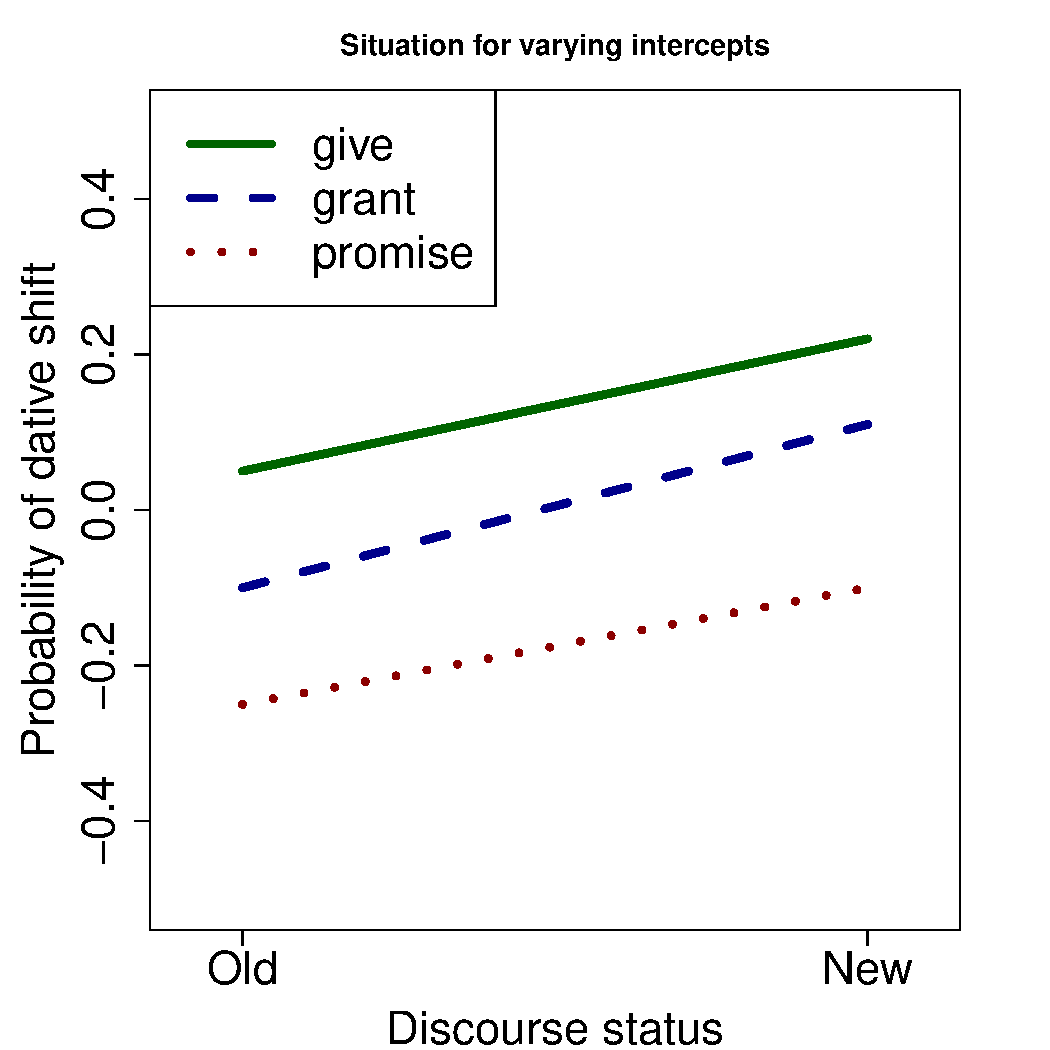
\includegraphics[width=0.5\textwidth]{graphics/var_int}~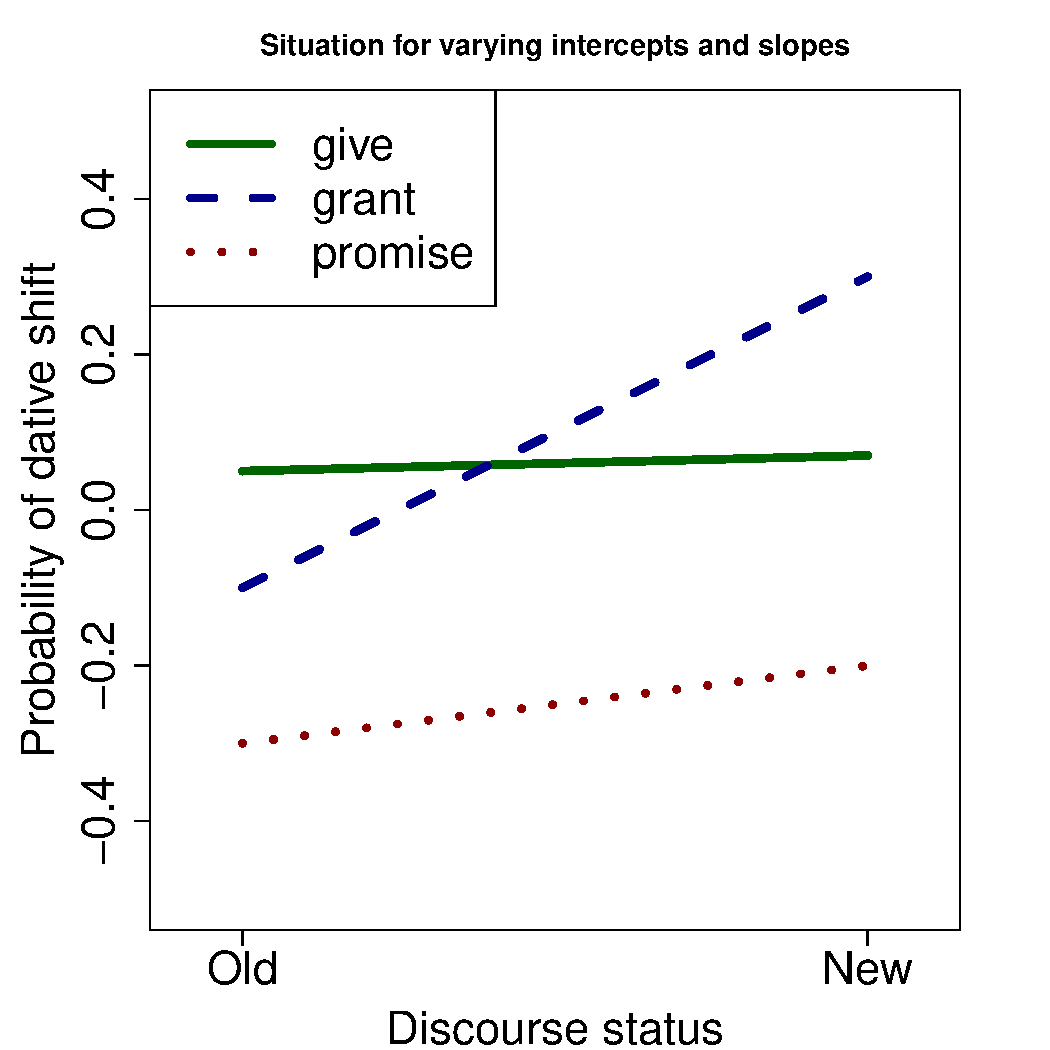
\includegraphics[width=0.5\textwidth]{graphics/var_int_slope}
  \caption{Interaction plots of fictional data in situations for varying intercepts or varying intercepts and additional varying slopes}
  \label{fig:varintlsope}
\end{figure}

We assume that we are looking at an alternation phenomenon like the dative alternation, wherein we are interested in the probability that, under given circumstances, the dative shift construction is chosen.
In the examination of the data, it turns out that the probability of the dative shift changes for old and new dative NPs.
The verb lemma also influences the probability of either variant being used.
The situation can now be as in the left or the right panel of Figure~\ref{fig:varintlsope}.
In the situation depicted in the left panel, the overall level in probability changes with the verb lemma, but for each verb lemma, the values change roughly by the same amount in exemplars with old and new dative NPs.
Note that the lines are not perfectly parallel because the figure is supposed to be an illustration of a data set rather than a fitted model, and we always expect some chance variation in data sets.
In the situation depicted in the right panel, however, the overall tendency also varies between lemmas, but additionally the lemma-specific tendencies also vary between exemplars with old and new NPs.
This is in fact nothing but an interaction between two factors (verb lemma and givenness), and we could use a fixed-effect interaction to take it into account.
However, if the verb lemma factor is used as a random effect grouping factor, the interaction is modeled as a so-called ``random slope''.
In Section~\ref{sec:modelspecificationandmodelingassumptions}, it is shown how all the different types of data sets discussed so far can be modeled using fixed effects models or, alternatively, using mixed effects models.
Which one is more appropriate will be argued to be better understood as a technical rather than a conceptual question.


\subsection{Model specification and modeling assumptions}
\label{sec:modelspecificationandmodelingassumptions}

In this section, it is discussed how the specification of mixed models differs from that of fixed effects models, and that for each model with random effects there is an alternative model with only fixed effects.
A major focus is on the question of when to use fixed and random effects.
The amount of technicality and notation is kept at the absolute minimum.
Particularly, the specification of models in mathematical notation is not always shown, and models are introduced in R notation.
For an appropriate understanding of model specification, readers should consult a more in-depth text book, for example Part~2A of \citet{GelmanHill2006} (pp.~235--342).
Without any knowledge of the mathematical notation conventions, it is impossible to understand many advanced text books and much of the valuable advice available online.

\subsubsection{Simple random intercepts}
\label{sec:simplerandomintercepts}

Readers with experience in fixed effects modeling should be able to see that a grouping factor encoding the verb lemma and all the other potential grouping factors discussed in the previous sections could be specified as normal fixed effects in a GLM.
This section introduces the main difference between the fixed-effect approach and the random-effect approach.
Logistic regression examples are used throughout this section, and we begin with the fictional corpus study of the dative alternation introduced in Sections~\ref{sec:hierarchicalormultilevelmodels} and \ref{sec:randominterceptsandslopes}.

First, we specify a minimal model with only the \textit{Lemma} grouping factor and one other predictor, namely \textit{Givenness}, both as fixed effects.

\begin{lstlisting}
  alternation.model <- glm(Construction~1+Lemma+Givenness,
                           data=alternation.data,
                           family=binomial(link=logit))
\end{lstlisting}

In the case of logistic regression in alternation modelling, \textit{Construction} is binary (levels 0 or 1, corresponding to the two alternants).
Furthermore, \textit{Lemma} has $m$ levels (one for each lemma), and \textit{Givenness} is also binary (levels 0 and 1, corresponding to \textit{not given} and \textit{given}).
A model specification like this encodes a theoretical commitment to what the researcher thinks is the mechanism that determines which alternant is chosen.
Concretely, it encodes the assumption that the probability of the outcome which is labeled as 1 can be predicted from the additive linear term specified as \textit{1+Lemma+Givenness}.
Because the influence of the regressors on the outcome is not linear in many cases, the additive linear term is transformed through the link function, here given as the inverse logit function in the \textit{family} parameter of the \textit{glm} function together with the specification of the distribution of the residuals (assumed to be binomial).
For logistic regression models, we assume that the distribution of the prediction errors follows the binomial distribution.
If another distribution (such as the Poisson distribution) and another link function (such as the logarithm, which is the default for Poisson models) is chosen, the specification of the model formula remains the same in R.

In any type of GL(M)M, the additive linear term consists of a number of sub-terms which are simply added up.
Each of these sub-terms (except for the intercepts) consists of the multiplication of the (estimated) \textit{coefficient} with an observed \textit{value} of one of the variables.
However, R notation for model formulæ simplifies the specification of the actual linear term.
First of all, the \texttt{1} in \texttt{Construction~1+Lemma+Givenness} is R's way of encoding the fact that an \textit{intercept} is part of the model.
An intercept is a constant sub-term to which all other sub-terms are added, and it can be seen as the reference value when all other sub-terms (corresponding to categorical or numeric regressors) assume 0 as their value.

For binary regressors like \textit{Givenness}, the only coefficient that is estimated directly encodes the value added to (in case of a positive coefficient) or subtracted from (in case of a negative coefficient) the linear term when the value of the regressor is 1 (in the example, when the referent is given).
When the value of the regressor is 0 (for example, when the referent is not given), 0 is added to the intercept.
The intercept thus encodes (among other things) something like a default for a binary regressor.
If the default corresponds to, as in the example, non-givenness, phrases like ``non-givenness is on the intercept'' or ```givenness equals zero' is on the intercept'' are often used.

\begin{table}
  \centering
  \begin{tabular}{cccc}
    \toprule
    \multicolumn{4}{l}{\textbf{Value of\ldots}} \\
    \textbf{Lemma} & $\mathbf{l_1}$ & $\mathbf{l_2}$ & $\mathbf{l_3}$ \\
    \midrule
    1 & 0 & 0 & 0 \\ 
    2 & 1 & 0 & 0 \\ 
    3 & 0 & 1 & 0 \\ 
    4 & 0 & 0 & 1 \\ 
    \bottomrule
  \end{tabular}
  \caption{Dummy coding of a categorical variable \textit{Lemma} with four levels, resulting in the binary dummy variables $l_1,l_2,l_3$}
  \label{tab:dummy}
\end{table}

However, a grouping factor such as \textit{Lemma} is usually a categorical variable with more than two levels.
In such a case, the $m$ levels of the grouping factor are \textit{dummy-coded}, and for all but one of these binary dummy variables, a coefficient is estimated.
Dummy coding is a way of encoding a categorical variable as a number of binary variables (see Table~\ref{tab:dummy}), and R takes care of dummy-coding automatically.
Because the first of the $m$ levels of the grouping factor is encoded by all dummy variables assuming the value 0, only $m-1$ sub-terms are added to the model, which means that only $m-1$ coefficients have to be estimated.
The first level of the grouping factor is thus ``on the intercept'' and becomes the reference to which all other levels are compared.%
\footnote{Picking one dummy as a reference level is necessary because otherwise infinitely many equivalent estimates of the model coefficients exist as one could simply add any arbitrary constant to the intercept and shift the other coefficients accordingly.
However, the estimator works under the assumption that there is a unique maximum likelihood estimate.
This extends to any other appropriate coding for categorical grouping variables.
}

To sum up and clarify, if in a given study \textit{Lemma} has four levels dummy-coded as $l_1$, $l_2$, $l_3$, and \textit{Givenness} is binary and coded as $g$ with $g=1$ if the referent is given, the formula corresponding to (\ref{eq:001}) looks like (\ref{eq:001a}) in mathematical notation, where the linear additive term is enclosed in $[ ]$, each sub-term appears in $( )$, and $c$ encodes the choice of the two alternants.

\begin{equation}
  Pr(c=1)=logit^{-1}\left[\alpha_0+(\beta_{l_1}\cdot l_1)+(\beta_{l_2}\cdot l_2)+(\beta_{l_3}\cdot l_3)+(\beta_{g}\cdot g)\right]
  \label{eq:001a}
\end{equation}

In plain English: the probability $Pr$ that the alternant of the construction coded as $1$ is chosen $Pr(c=1)$ is calculated as the inverse logit of the linear term.
The linear term is just the sum of the intercept $\alpha_0$ and the measured values, each multiplied by its corresponding coefficient labelled $\beta$.

In such a model, the effect of each verb lemma is treated as a fixed population parameter, just like the effect of givenness.
In other words, the algorithm which estimates the coefficients for the $m-1$ dummy variables tries to find a fixed value for each of them without taking the variation between them into account.
With many levels, this requires a lot of data, and levels for which only a few observations are available in the data set have very imprecise coefficient estimates with large confidence intervals.

This is where random effects come into play as an alternative.
If we treat the same grouping factor as a random intercept, we let the intercept vary by group, \ie\ each group is allowed to have its own intercept.
Furthermore, we give the varying intercepts a (normal) distribution instead of estimating $m-1$ fixed population parameters.
This means that the group-wise intercepts are assumed to be normally distributed around $0$.
This and nothing else is the conceptual difference between a fixed effect and a random effect.%
\footnote{There is one other practical difference.
If models are used to make actual predictions (which is rarely the case in linguistics), a random effect allows one to make predictions for unseen groups.
See \citet[272--275]{GelmanHill2006}.}

In R, the model specification then looks as follows, where ``1|'' can be read as ``an intercept varying by''.

\begin{lstlisting}
  alternation.model <- glmer(1+Givenness+(1|Lemma),
                             data=alternation.data,
                             family=binomial(link=logit))
\end{lstlisting}

The sub-term \textit{Givenness} remains the same as in the GLM specification above, and it is still treated as a fixed effect.
The sub-term \textit{(1|Lemma)} encodes that an intercept will be added to the linear term depending on which lemma is observed.
This is obvious in mathematical notation corresponding to the above R code as shown in (\ref{eq:002a}).
In addition to the overall intercept $\alpha_0$, there is another constant term $\alpha_{[Lemma]}$, which is chosen appropriately for each level of \textit{Lemma}.

\begin{equation}
  Pr(c=1)=logit^{-1}\left[\alpha_0+\alpha_{[Lemma]}+(\beta_{g}\cdot g)\right]
  \label{eq:002a}
\end{equation}

Crucially, instead of estimating a batch of $m-1$ coefficients for the levels of the grouping variable, a varying intercept (assumed to come from a normal distribution) is predicted for each of its $m$ levels.
Essentially, this means that the varying intercepts are predicted from their own linear model.
All more complex model structures to be discussed below are extensions of this approach.

\subsubsection{Choosing between random and fixed effects}
\label{sec:choosingbetweenrandomandfixedeffects}

One commonly given reason to use a random effect instead of a fixed effect is that ``the researcher is not interested in the individual levels of the random effect'' (or variations thereof).
Such recommendations should be taken with a grain of salt.
\citet[245--247]{GelmanHill2006} summarise this as well as other diverging and partially contradicting recommendations for what should be a random effect as found in the literature.
They conclude that there is essentially no universally accepted and tenable conceptual criterion of deciding what should be a random effect and what a fixed effect.
The author of this chapter agrees with their conclusion that random effects should be preferred whenever it is technically feasible.
Understanding when it is technically feasible requires at least some understanding of two major points.
First, the variance in the intercepts needs to be estimated if a random effect is used.
Second, the random intercepts can be understood as a compromise between fitting separate models for each group of the grouping factor (\textit{no pooling}) and fitting a model while ignoring the grouping factor altogether (\textit{complete pooling}), see \citet[Ch.~12]{GelmanHill2006}.

As was stated above, the random intercepts are assumed to come from a normal distribution, and therefore the variance between them has to be estimated with sufficient precision.
From the estimated variance and the data for a specific group, the estimator predicts the \textit{conditional mode} in a GLMM or the \textit{conditional mean} in a LMMs for that group (see \citealt[Ch.~1]{Bates2010}).
The conditional mode\slash mean for a group is the value of the varying intercept for this group.
It is the numerical value shown by R packages like \texttt{lme4} for each level of a random intercept variable.
This procedure, however, requires that the number of groups must not be too low.
As a rule of thumb, if there are fewer than five levels, a grouping factor should be included as a fixed effect, regardless of its conceptual interpretation.
Although one often finds default recommendations telling practitioners to use a speaker grouping variable as a random effect, it would be ill-advised to do so if there are exemplars from less than five speakers in the sample.
Along the same lines, the distinction between intersective and non-intersective adjectives (Section~\ref{sec:crossedandnestedeffects}) is not a suitable grouping factor for use as a random effect because it has too few levels.
Hence, if such a grouping factor is used in a model where it nests finer-grained groups of another factor (such as adjective lemmas), the nested factor with the low number of levels should be used as a second-level fixed effect rather than a nesting random effect.

If the number of groups is reasonably large, the next thing to consider is the number of observations per group.
Alternatives to using a random effect would be to estimate a separate model for each level of the grouping factor, or to include it as a fixed effect.
In both cases the effects are not treated as random variables, and fixed coefficients per group are estimated without taking the between-group variance into account.
With a random effect, however, the conditional modes\slash means are pulled (\textit{shrunken}) towards the overall intercept (\textit{shrinkage}).
When the number of observations in a group is low, the conditional mode\slash mean is simply shrunken more strongly towards $0$, predicting only a small deviation from the overall tendency.%
\footnote{Terminologically, shrinkage is thus \textit{stronger} (and the conditional mode\slash mean is closer to $0$) if there is less evidence that a group deviates from the overall tendency.
The lower the number of observations per group, the lesser evidence there is.}
On the other hand, fixed effect estimates would become inexact and would probably be dismissed because of growing uncertainty in the estimate (large confidence intervals, high p-values) when the number of observations for a level is low.
Thus, low numbers of observations in all or some groups are often detrimental for using fixed effects grouping factors.
Random effects are much more robust in such situations because of shrinkage.
On the downside, a conditional mode that was strongly shrunken (due to a low number of observations) cannot be distinguished straightforwardly from a conditional mode of a group which simply does not deviate a lot from the average tendency.
For fixed effects, we have both a parameter estimate and a possible significance test, but for random effects, we only have the prediction of the conditional mode\slash mean.
However, so-called \textit{prediction intervals} can be calculated for individual per-group intercepts, and we return to them in the following section.


\subsubsection{Model quality and model selection}
\label{sec:significancetestingandcoefficientsofdetermination}

\paragraph{Significance}

It is not adequate to do any kind of significance testing on the individual levels of the random effect because they are not estimates in the conceptual and technical sense.%
\footnote{Again, we do not assume them to be fixed population parameters, which would be the case for true estimates such as fixed effects coefficients.}
There are ways of calculating \textit{prediction intervals} (which are not the same as confidence intervals) for conditional modes in order to specify the quality of the fit (see Section~\ref{sec:practicalguidewithr}), but they should not be misused for talking about significance.
Not doing significance tests for single levels of the grouping factor does, however, not mean that the researcher is not interested in the individual conditional modes, which is proven by the fact that they are often reproduced in research papers, for example in the form of a dot plot.
Also, we can still get a good idea of the per-group tendencies by looking at the conditional modes\slash means.
Additionally, a random effect allows the researcher to quantify the between-group variance, which is not possible for fixed effects.

\paragraph{Relevance of the random effects}

A related question is whether the inclusion of the random effect improves the model quality.
It is recommended here to include all random effects as required by the design of the study (after having decided based on the criteria given in Section~\ref{sec:choosingbetweenrandomandfixedeffects} whether they should be random rather than fixed).
Only if they clearly (and beyond doubt) have no effect, practitioners should consider removing them.
To check whether they have an effect, the estimated between-group variance is the first thing to look at.
If it is close to $0$, there is most likely not much going on between groups, or there simply was not enough data to estimate the variance.
In LMMs, it is possible to compare the residual (item-level) variance with the between-group variance to see which one is larger, and to which degree.
If, for example, the residual variance is 0.2 and the between-group variance is 0.8, then we can say that the between-group variance is four times larger than the residual variance, which would indicate that the random effect has a considerable impact on the response.
This comparison is impossible in GLMMs because their (several types of) residuals do not have the same straightforward interpretation as those of LMMs.

Furthermore, models can be compared using likelihood ratio (LR) tests.
In such tests, a model including the random effect and a model not including it are compared, similar to LR tests for the comparison of fixed effects.
Such pairs of models, where one is strictly a simplification of the other, are called \textit{nested models} (not to be confused with \textit{nested effects} discussed in Section~\ref{sec:crossedandnestedeffects}).
A sometimes more robust alternative to the ordinary LR test are parametric bootstrap tests. 

With all this, it should be kept in mind that it is \textit{never} appropriate to make formal comparisons between a GLMM with a random effect and a GLM with the same factor as a fixed effect using any test or metric (including so-called information criteria such as Akaike's or Bayes').
\textit{Informally} comparing coefficients of determination ($R^2$) between such pairs of models has a limited use, as will be shown below.

\paragraph{Quality of the fit}

To measure how well a GLMM fits the data, any metric that is based on prediction accuracy can be used in the same way as with GLMs.
For example, the rate of correct predictions on the data used for model estimation or cross-validation methods are appropriate.

Coefficients of determination (pseudo-$R^2$) can be used to give some idea of the overall model fit.
For GLMMs, \citet{NakagawaSchielzeth2013} have proposed a method that distinguishes between \textit{marginal} $R^2$ (only fixed effects) and \textit{conditional} $R^2$ (fixed and random effects).
This has become a de facto standard.
In cases where an effect works well as a fixed or a random effect (for example, if it has between five and ten levels with enough data points for each level), the marginal and conditional $R^2$ measures for the GLMM converge in an expected way with Nagelkerke's $R^2$ for corresponding GLMs.
The marginal $R^2$ for a GLMM estimate is roughly the same as Nagelkerke's $R^2$ for a GLM estimate where the grouping factor is ignored.
Also, the conditional $R^2$ for a GLMM estimate is roughly the same as Nagelkerke's $R^2$ for a GLM estimate which includes the grouping factor as a fixed effect.


\subsubsection{More complex models}
\label{sec:morecomplexmodels}

\paragraph{Varying intercepts and slopes}

In Section~\ref{sec:randominterceptsandslopes}, it was shown under which conditions a varying-intercept and varying-slope (VIVS) model might be useful.
While it is possible to have just a varying slope, this is rarely useful, and we discuss only varying-intercept and varying-slope (VIVS) models.

A random slope is a good choice when the strength or direction of some fixed effect varies by group.
We extend the simple model from (\ref{eq:001}) to include random slopes for \textit{Givenness} varying by \textit{Lemma} using R notation in (\ref{eq:003}).
Each variable from the fixed effects part of the formula which we expect to vary by \textit{Lemma} is simply repeated before the | symbol.

\Rformula{Construction}{1+Givenness+(1+Givenness|Lemma)}{eq:003}

With this model specification, a fixed coefficient for \textit{Givenness} will still be estimated.
However, an additional value will be predicted for each lemma, and this value has to be added to the fixed coefficient.
In mathematical notation, this is very transparent, as shown in (\ref{eq:003a}).
The varying slope for \textit{Givenness} to be chosen appropriately for each \textit{Lemma} is specified as $\beta_{g[Lemma]}$.

\begin{equation}
  Pr(c=1)=logit^{-1}\left[\alpha_0+\alpha_{[Lemma]}+((\beta_{g}+\beta_{g[Lemma]}) \cdot g)\right]
  \label{eq:003a}
\end{equation}

A source of problems in VIVS models is the fact that in addition to the variance in the intercepts and slopes, the covariance between them has to be estimated.
If in groups with a higher-than-average intercept, the slope is also higher than average, they are positively correlated, and vice versa.
These relations are captured in the covariance.
Technically speaking, the joint distribution of the random intercepts and the random slopes is assumed to follow a multivariate normal distribution with means, variances, and covariances to be estimated.
The number of variance parameters to be estimated thus obviously increases with more complex model specifications, and the estimation of the parameters in the presence of complex variance-covariance matrices requires considerably more data than estimating a single variance parameter.
The estimator algorithm might terminate, but typically covariance estimates of $-1$ or $1$ indicate that the data was too sparse for a successful estimation of the parameter.
In this case, the model is \textit{over-parametrised} and needs to be simplified (see \citealt{BatesEa2015a,MatuschekEa2017}).

\paragraph{Nested and crossed random effects}

The difference between nested and crossed random effects is only defined when there are two or more random effects.
As it was explained in Section~\ref{sec:crossedandnestedeffects}, nested random effects are appropriate tools when the levels of a grouping factor are nested within the levels of another grouping factor.
Technically, while varying slopes can be understood as interactions between a fixed and a random effect, nested random intercepts can be understood as interactions between two or more random effects.
Crossed random effects are just several unrelated random effects.

In the model specification (both in R notation and in mathematical notation), there is no difference between a crossed and a nested random effect.
Both are specified like independent random effects.
See (\ref{eq:004}) for an example in R notation which extends (\ref{eq:002}).

\Rformula{Construction}{1+Givenness+(1|Lemma)+(1|Semantics)}{eq:004}

In (\ref{eq:004}), \textit{Semantics} could be a factor encoding the semantic classes which nest individual lemmas.
It could also be a (crossed) grouping factor completely unrelated to the lemmas, for example encoding some semantic property of the whole sentence containing the construction.
As was mentioned in Section~\ref{sec:crossedandnestedeffects}, the question on the practitioner's side is rather how the data are organised.
If the data have a nested structure, the estimator will treat them as nested, otherwise as crossed.
Data have a nested structure whenever each level of a (nesting) random effect can always be determined entirely from the levels of another (nested) factor.


\paragraph{Second-level predictors}

In Section~\ref{sec:hierarchicalormultilevelmodels}, situations were introduced where the random effects themselves can be partially predicted from second-level fixed-effects.
In R notation, the true model structure is entirely blurred, and practitioners even run the risk of working with second-level predictors without realising it.

We extend (\ref{eq:002}) to (\ref{eq:005}) by adding a numeric fixed effect which specifies the token frequency for each level of \textit{Lemma}.

\Rformula{Construction}{1+Givenness+Lemmafrequency+(1|Lemma)}{eq:005}

This is the only way to specify second-level predictors in standard R notation.
The data set has to be organised as shown in Table~\ref{tab:multilevel}, where for each data point a level of \textit{Lemma} is specified and the appropriate frequency value for this level of \textit{Lemma} is given in a separate column.%
\footnote{There are, of course, elegant ways of pulling the frequency values from another data frame on the fly in R.}
R treats \textit{Lemmafrequency} as a second-level predictor automatically under such conditions.
Simply speaking, this means that the random intercept for \textit{Lemma} will now be predicted from its own linear model.
In Section~\ref{sec:practicalguidewithr}, a model with second-level effects will be used for illustration purposes.




\section{Practical guide with R}
\label{sec:practicalguidewithr}

\subsection{Specifying models using \texttt{lme4} in \texttt{R}}
\label{sec:specifyingmodelsusinglme4inr}

This section and the next focus on \texttt{lme4}, an often used package to do multilevel modeling in \texttt{R} with maximum likelihood methods \citep{BatesEa2015}.
The data set used to illustrate the process of fitting GLMMs in \texttt{R} is taken from \citet{Schaefer2018}.

\subsubsection{Overview of the data set}

The data used here for illustration purposed is used in \citet{Schaefer2018} to model a binary case alternation in German measure phrases.
In the first alternant, the kind-denoting noun (here \textit{Wein} `wine') is assigned the same case as the head measure noun as in (\ref{ex:intro:alternation1}).
In the second alternant, the kind-denoting noun is in the genitive as in (\ref{ex:intro:alternation2}).

\begin{exe}
  \ex\label{ex:intro:alternation}
  \begin{xlist}
    \ex[ ]{\label{ex:intro:alternation1} \gll Wir trinken [[ein Glas]\Sub{Acc} [guten Weins]\Sub{Gen}]\Sub{Acc}.\\
    we drink a glass good wine \\
    \glt We drink a glass of good wine.}
    \ex[ ]{\label{ex:intro:alternation2} Wir trinken [[ein Glas]\Sub{Acc} [guten Wein]\Sub{Acc}]\Sub{Acc}.}
  \end{xlist}
\end{exe}

The influencing first-level factors derived from theory-driven analysis and previous accounts comprise the numeric stylistic indicator variables \texttt{Badness} and \texttt{Genitives}, a binary variable \texttt{Cardinal} encoding whether the NP is modified by a cardinal or not, and the three-level variable \texttt{Measurecase} encoding the case of the head noun.
Furthermore, there are two crossed random intercepts for the kind noun (\texttt{Kindlemma}) and the measure noun (\texttt{Measurelemma}).
These random intercepts come with second-level models including a number of fixed second-level effects.
For \texttt{Kindlemma}, there are: \texttt{Kindfreq} (numeric, z-transformed), which encodes the lemma frequency; \texttt{Kindgender} (binary), which encodes the grammatical gender of the kind noun; \texttt{Kindattraction} (numeric, z-transformed), which encodes the influence of neighbouring constructions.
For \texttt{Measurelemma}, there are: \texttt{Measurefreq} and \texttt{Measureattraction}, which correspond to the similarly named variables for \texttt{Kindlemma}; \texttt{Measureclass} (5-level categorical) which encodes the broad semantic class of the measure noun.

\subsubsection{A simple varying intercept instead of a fixed effect}

\paragraph{Fitting and evaluating the model}

First, it is shown how a grouping factor can be specified as a fixed or a random effect.
The following is the standard \texttt{glm()} call to estimate a model with the measure lemma (150 levels) as a fixed effect.

\vspace{0.5\baselineskip}

\begin{lstlisting}
glm.01 <- glm(Construction~1
              +Measurelemma
              +Badness
              +Cardinal
              +Genitives
              +Measurecase,
	      data=measure,
	      family=binomial(link=logit))
\end{lstlisting}

The output of the \texttt{summary(glm.01)} command (not shown here) shows that the estimates for the 149 fixed effects corresponding to \texttt{Measurelemma} have extremely high standard errors and are virtually unusable.
The Nagelkerke coefficient of determination for this model can be calculated using the \texttt{MagelkerkeR2(glm.01)} function from the \texttt{fmsb} package, and it is 0.397.

However, the grouping factor \texttt{Measurelemma} is not suitable for use as a fixed effect, and the following specification re-estimates the model as a GLMM using the \texttt{glmer} function with \texttt{Measurelemma} as a varying intercept (assuming that the \texttt{lme4} package was loaded).

\vspace{0.5\baselineskip}

\begin{lstlisting}
glmm.01 <- glmer(Construction~1
                 +(1|Measurelemma)
                 +Badness
                 +Cardinal
                 +Genitives
                 +Measurecase,
                 data=measure,
		 family=binomial(link=logit))
\end{lstlisting}

The output of the \texttt{summary(glmm.01)} command looks as follows (abbreviated).

\vspace{0.5\baselineskip}

\begin{lstlisting}
Random effects:
 Groups       Name        Variance Std.Dev.
 Measurelemma (Intercept) 1.252    1.119   
Number of obs: 5063, groups:  Measurelemma, 150

Fixed effects:
               Estimate Std. Error z value Pr(>|z|)    
(Intercept)    -2.32135    0.17867 -12.992  < 2e-16 ***
Badness        -0.14065    0.04474  -3.144  0.00167 ** 
CardinalNo      1.35673    0.13947   9.727  < 2e-16 ***
Genitives      -0.73886    0.04239 -17.429  < 2e-16 ***
MeasurecaseAcc -0.01923    0.08821  -0.218  0.82740    
MeasurecaseDat  0.25047    0.12045   2.079  0.03758 *  
\end{lstlisting}

Besides the standard coefficient table for the fixed effects including the overall intercept.
Above this coefficient table, there is a summary of the random effects.
The number of groups for \texttt{Measurelemma} is correctly given as 150, and the variance in the random intercepts is 1.252.%
\footnote{The variance-covariance matrix of GLMMs can also be extracted directly using the \texttt{VarCorr(glmm.01)} command from \texttt{lme4}.}
As a rule of thumb, the larger is the variance between the intercepts, the larger are the differences between the groups.
For the variance estimate, confidence intervals can be obtained with either one of the following commands, where the first one uses the profile method (based on likelihood ratio tests) and the second one uses the parametric bootstrap, which is sometimes considered more robust.%
\footnote{Since the bootstrap (especially with smaller original sample sizes tends to run into replications where the estimation of the variance fails and is thus returned as 0, the bootstrap interval is sometimes skewed towards 0 when the profile confidence interval frames the true value symmetrically. The bootstrap is thus not always more robust or intrinsically better.
Comparing both methods is recommended.}

\vspace{0.5\baselineskip}

\begin{lstlisting}
confint(glmm.01, parm="theta_", method="profile")
confint(glmm.01, parm="theta_", method="boot", nsim = 250)
\end{lstlisting}

For the first command, the output (95\% confidence interval) is 0.887 and 1.414.
Without applying formal significance testing, this is a reasonably narrow interval, and it does not include 0.
It is generally not a good idea to do (stepwise) model selection for random effects.
Even worse, while bootstrap methods are available for the comparison of two nested mixed models (see below), the comparison of a GLM and a GLMM (which extends the GLM by one random effect) is mostly uncharted territory and should be avoided.

Single conditional modes for the levels of the grouping factor can be extracted using the \texttt{ranef} command.
The following command stores a list of conditional modes for \texttt{Measurelemma} in \texttt{glmm.01.ranef}.

\vspace{0.5\baselineskip}

\begin{lstlisting}
glmm.01.ranef <- ranef(glmm.01, condVar = TRUE,
                       drop = TRUE)$Measurelemma
\end{lstlisting}

If the options \texttt{condVar = TRUE} and \texttt{drop = TRUE} are passed as above, then conditional variance-covariance estimates are returned as attributes of the result.
They have to be accessed using the \texttt{attribute} function as shown below.

\vspace{0.5\baselineskip}

\begin{lstlisting}
attributes(glmm.01.ranef)$postVar
\end{lstlisting}

These can be used to construct prediction intervals around the predicted conditional modes in order to display them in tabular form or plot them-
While some ready-made functions exist to plot them in the form of a dot plot, it is good to have a custom plotting function.
If the random effect has many levels, it might only be possible to plot a selection (random or informed) of the conditional modes.
The \texttt{R} script accompanying this chapter contains a maximally simple example using only standard plotting functions which creates a dot plot with prediction intervals for a random subset of the conditional modes.
An example is given in Figure~\ref{fig:condmodes}, where the smaller prediction intervals correspond strongly to the number of exemplars observed in the different groups.

\begin{figure}
  \centering
  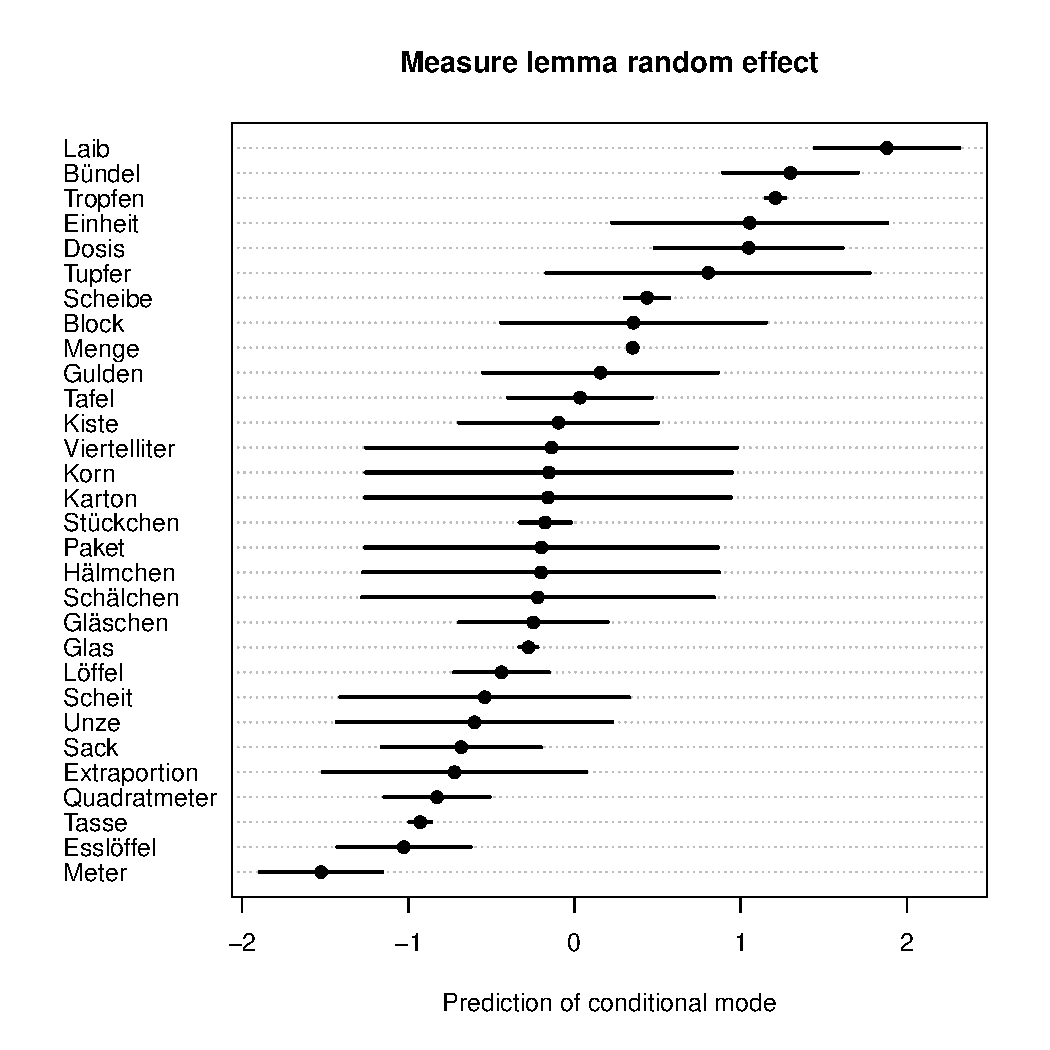
\includegraphics[width=\textwidth]{RPHCL/ranef_selection}
  \caption{Dot plot with prediction intervals for a random subset of 30 conditional modes (model \texttt{glmm.01}, random intercept for \texttt{Measurelemma})}
  \label{fig:condmodes}
\end{figure}

Turning to the quality of the overall model fit, Nakagawa \& Schielzeth's coefficients of determination can be calculated with the \texttt{r.squaredGLMM(glmm.01)} command (from the \texttt{MuMIn} package).
The output looks as follows.

\vspace{0.5\baselineskip}

\begin{lstlisting}
      R2m       R2c
0.2004865 0.4209018
\end{lstlisting}

This informs the user that the fixed effects cumulatively account for a proportion of 0.200 of the total variance in the data.
Taking also the random effect into account, the model explains a proportion of 0.421 of the total variance.
The random effect thus appears to be relevant.
Comparing the conditional $R^2$ to the Nagelkerke $R^2$ of the GLM with \texttt{Measurelemma} as a fixed effect (which was 0.397), we see that the difference is not substantial although the individual coefficient estimates in the GLM were unreliable.

Furthermore, readers are encouraged to compare the estimates of the fixed effects for \texttt{glm.01} (except \texttt{Measurelemma}) and for \texttt{glmm.01}.
The coefficient estimates (except for the intercept, which is heavily offset in \texttt{glm.01}) themselves do not differ much between the GLM and the GLMM, which indicates that the grouping variable \texttt{Measurelemma} does not enter into an interaction with the fixed effects.
However, the standard deviations (and consequently the confidence intervals as well as the p-values) change.

\paragraph{Reporting the results}

Journals and conferences in corpus linguistics apparently do not enforce strict guidelines when it comes to reporting the results of GLMM fits.
While a coefficient table for the fixed effects is a de-facto standard for GLMMs just as much as for GLMs, there is no such de-facto standard with regard to which measures of model quality for GLMMs should be reported, and especially how random effects should be reported.
In addition to the coefficient table (and other diagnostics also recommended for GLMs such as variance inflation factors; \citealp{FoxMonette1992,ZuurEa2010}), which should at least contain the coefficient estimate, the standard error, and (possibly bootstrapped) confidence intervals for the fixed effects, the present author recommends to report (either in the running text, in tabular form, or in the caption of the coefficient table):

\begin{enumerate}
  \item the estimate of the random effect variance (and covariance) parameters
  \item (bootstrap) confidence intervals for the above
  \item Nakagawa \& Schielzeth's $R^2$ coefficients of determination
  \item optionally all or some conditional modes with prediction intervals in tabular form or as a dotplot (see Figure~\ref{fig:condmodes})
  \item (bootstrap) p-values for random effects (if absolutely necessary, and only if the model comparison is possible between nested GLMMs and does not involve the direct comparison of a GLM and a GLMM)
\end{enumerate}

\subsubsection{More complex models}

The \texttt{glmer} call as used for the original paper is as follows.

\vspace{0.5\baselineskip}

\begin{lstlisting}
glmm.10 <- glmer(Construction~1
                 +(1|Measurelemma)   # Random.
                 +(1|Kindlemma)
                 +Badness            # Item-level.
                 +Cardinal
                 +Genitives
                 +Measurecase
                 +Kindattraction     # Kind lemma level.
                 +Kindfreq
                 +Kindgender
                 +Measureattraction  # Measure lemma level.
                 +Measureclass
                 +Measurefreq,
                 data=measure,
		 family=binomial(link=logit),
		 na.action = na.fail,
                 control=glmerControl("bobyqa"))
\end{lstlisting}

Since the model has a relatively high degree of complexity, the option \texttt{control=glmerControl("bobyqa")} is required.
It selects a different optimiser, which is an algorithm used by the estimator.
In general, BOBYQA optimisers are highly robust, and using a BOBYQA is the first step to try when there are convergence errors.

The second-level effects have the same value for each level of the corresponding random intercept and are automatically treated as second-level effects.
In order to illustrate the interpretation of the conditional modes and the fixed effects coefficients in such a model, there is code in the accompanying script which extracts all relevant values and calculates a predicted value for item 99 from the \texttt{measure} data set.
For example, the overall intercept of -3.653 can be extracted via the following command.

\vspace{0.5\baselineskip}

\begin{lstlisting}
coef(summary(glmm.03))['(Intercept)','Estimate']
\end{lstlisting}

To this intercept, the sub-terms for first-level fixed effects are added.
They can be calculated as follows, using \texttt{Badness} as an example.
The result is 0.0183.

\vspace{0.5\baselineskip}

\begin{lstlisting}
coef(summary(glmm.03))['Badness', 'Estimate'] *
  measure[99, 'Badness']
\end{lstlisting}

In other words, we extract the fixed-effect coefficient estimate for \texttt{Badness} and multiply it with the \texttt{Badness} value observed for item 99.

In order to calculate the contribution of the second-level effects, which will be added to the overall intercept and the first-level fixed-effects sub-terms, we first need to extract the appropriate group-level intercept.
The following code extracts the \texttt{Kindlemma} random intercept for item 99, which is -0.159 for the lemma \textit{Wasser} `water'.

\vspace{0.5\baselineskip}

\begin{lstlisting}
ranef(glmm.03)$Kindlemma[
  as.character(measure[99, 'Kindlemma']), '(Intercept)']
\end{lstlisting}

To these group-level intercepts, the second-level fixed-effects sub-terms are added, and they can be calculated very much like their first-level equivalents.
For example, the following code calculates the sub-term for \texttt{Kindfreq}, which is -0.044 (the logarithmised frequency per one million tokens of \textit{Wasser}) in this case.

\vspace{0.5\baselineskip}

\begin{lstlisting}
coef(summary(glmm.03))['Kindfreq', 'Estimate'] *
  measure[99, 'Kindfreq']
\end{lstlisting}

All in all, the prediction for the \texttt{Measurelemma} second-level model is -0.027.
For the \texttt{Kindlemma} second-level model, it is 0.125, and for the first-level fixed-effects part of the model (including the overall intercept), it is -3.382.
Added up, the linear term is predicted to be -3.284.
This result needs to go through the inverse logit link function (implemented as \texttt{invlogit} in the \texttt{car} package, for example), which results in 0.036.
Given the coding of the response variable, this means that the model predicts a probability of 0.036 that the genitive construction is chosen in the given example.
Readers are advised to go through the full calculations in order to understand what the different numbers in their reported GLMMs represent.
They will likely realise that the superficial maths involved is relatively transparent, even for more complex models.


\newpage
\section{Representative studies}

\begin{mdframed}
  \subsection*{\citet{WolkEa2013}}
  
  \paragraph{Research questions}

  The authors aim to achieve two things.
  First, they want to compare changes in two word order-related alternations in the history of English between 1650 and 1999: the dative alternation and the genitive alternation.
  They look for influencing features shared in both cases as well as construction-specific features.
  Second, they aim to show that historical data fits well into a probabilistic, cognitively oriented view of language.

  \paragraph{Data}

  The authors use the \textsc{archer} corpus \citep{BiberEa1994}, which contains texts from various registers from 1650 to 1999.
  For both constructions, carefully designed sampling protocols were used (see their Section~4).
  For the annotation of the data, both available corpus meta data were used (text ID, register, time in fractions of centuries, centered at 1800) as well as a large number of manually coded variables (constituent length, animacy, definiteness, etc.).
  Furthermore, the possessor head lemma (genitive alternation) and the verb lemma (dative alternation) were coded.

  \paragraph{Method}

  Two mixed effects logistic regression models are estimated.
  For the genitive alternation, the text ID and the possessor head lemma are used as crossed random effects.
  The authors state on p.~399 that they collapsed all head noun lemmas with less than four occurrences into one category because otherwise ``difficulties'' would arise.
  However, it is the advantage of random effects modeling that it can deal with a situation where categories have low numbers of observations (see \textit{shrinkage}, Section~\ref{sec:choosingbetweenrandomandfixedeffects}).
  For the dative alternation, the model includes the text ID, the register (which nests the text ID) as well as the lemma of the theme argument and the verb. 

  \paragraph{Results}

  It is found that many factors have a shared importance in both alternations, \eg definiteness, animacy, construction length.
  It is also argued that the observed tendencies -- such as \textit{short-before-long} and \textit{animate referents first} -- are in line with synchronic corpus based and experimental findings about general cognitive principles underlying the framework of probabilistic grammar.
  These principles remain in effect, but the strength of their influence changes over time.

\end{mdframed}

\begin{mdframed}

  \subsection*{\citet{Gries2015}}

  \paragraph{Research questions}
  
  The paper is programmatic in nature.
  The author re-analyses data from a previously published study on verb particle placement in English.
  He uses a GLMM instead of a fixed-effects logistic regression to show that including random effects in order to account for variation related to mode, register, and subregister increases the quality and predictive power of the model.
  He also argues that by not doing so, corpus linguists risk violating fundamental assumptions about the independence of the error terms in models.
  
  \paragraph{Data}
  
  The data are $2,321$ instances of particle verbs showing either verb--direct object--particle or verb--particle--direct object order, taken from the ICE-GB.
  The grouping factors derived from the structure of the corpus are mode (only two levels), register (five levels), and subregister ($13$ levels).
  They are nested: mode nests register, which nests subregister.
  Additionally, verb and particle lemma grouping factors are annotated.
  Finally, two fixed effects candidates are annotated (the type of the head of direct object and the logarithmised length of the direct object in words).
  
  \paragraph{Method}
  
  The author uses the model selection protocol described in \citet{ZuurEa2009} to first find the optimal random effects structure using ANOVAs and AIC comparisons as well as analyses of the estimated variance for single random effects.
  He then goes on to find the optimal fixed effects structure.
  Additionally, he compares the pseudo-$R^2$ measure of the resulting mixed models.
  
  \paragraph{Results}

  Gries finds that the verb and particle lemma play and the subregister play a significant role.
  Notably, the variance estimate for mode is close to $0$ from the beginning of the model selection procedure.
  This is not surprising, as two levels are not nearly enough in order for the variance to be reliably estimated, and it could maybe be used as a second-level predictor instead (see Section~\ref{sec:choosingbetweenrandomandfixedeffects}).
  The $R^2$ values of the final model are very high, with a considerable difference between marginal $R^2_m=0.57$ and conditional $R^2_c=0.748$, which indicates that the random effects do in fact improve the model fit.
  It is also shown that the classification accuracy is considerably improved over that of a GLM without random effects, but differently for different lexical groups and subregisters.
  The paper thus shows that it is not appropriate to ignore lexical grouping factors and grouping factors derived from the corpus structure, especially as both are easy to annotate automatically.

\end{mdframed}



\section{Further reading}
\label{sec:furtherreading}

Chapters~1--15 and Chapters~20--24 of \citet{GelmanHill2006} are a highly recommended read, especially for \texttt{R} and \texttt{lme4} users.
Similarly, \citet{ZuurEa2009} has a reputation among \texttt{R} users of mixed effects models in many fields.
The companion to \texttt{lme4}, \citet{Bates2010} and the overview in \citet{BatesEa2015} are obligatory reads for users of \texttt{lme4}.

\printbibliography
%\bibliography{glmm}

\end{document} 
